\documentclass[10pt]{article}
\usepackage{graphicx}
\usepackage{amssymb}
\usepackage[fleqn]{amsmath}
\usepackage{nccmath}
\usepackage{cases}
\usepackage{hyperref}
\usepackage{multicol}
\usepackage{tikz}
\usepackage{tikz}
\usetikzlibrary{shapes.geometric}
\usepackage{pgfplots}
\usepackage{enumitem}
\pgfplotsset{compat=1.18}
\usepackage{float}
\usetikzlibrary{calc,angles}
\thispagestyle{empty}

\begin{document}
\section*{Gauss's Proof}
Gauss starts with a polynomial with real coefficients
\begin{align*}
    P(z)=a_0+a_1z+a_2z^2+\cdots+a_n z^n 
\end{align*}
All real polynomials can be reduced into a product of linear and irreducible quadratic factors.
For appropriate values of $r$ and $\phi$, a linear factor can be expressed as $z\pm r,r\ge 0$ and a quadratic factor can be expressed as $z^2+2r\cos\phi z+r^2,r>0$ with complex roots $r(\cos\phi\pm i\sin\phi)$.
Substituting $z=r(\cos\phi+ i\sin\phi)$ we define $2$ new polynomials \begin{align*}
    U(r,\phi)=a_0+a_1\cos(\phi) r+a_2\cos(2\phi) r^2+\cdots+a_n\cos (n\phi) r^n\\
    T(r,\phi)=a_1\sin(\phi) r+a_2\sin(2\phi) r^2+\cdots+a_n\sin (n\phi) r^n
\end{align*}
where $U(r,\phi)=Re(P(z))$ and $T(r,\phi)=Im(P(z))$.\\
Consider the curves $U=0$ and $T=0$. Our goal is find the intersection of these two curves within a sufficiently large circle of radius $R$. For if we can determine $(r,\phi)$ such that $U=0$ and $T=0$ simultaneously, then $z\pm r\mid P(z)$ or $z^2+2r\cos\phi z+r^2\mid P(z)$.\\
Gauss observes the behavior of the two curves inside the circle. By Bezout's lemma, $U=0$ and $T=0$ should each intersect the circle $2n$ times for a total of $4n$ intersections with the circle. 
      \begin{figure}[h]
        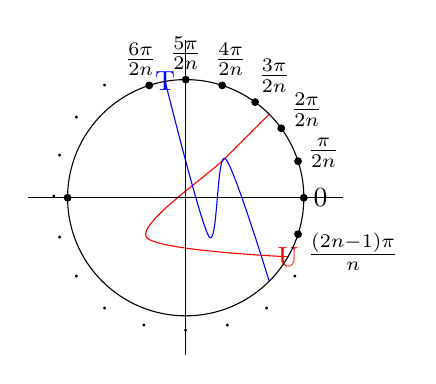
\begin{tikzpicture}
            \draw [red] plot [smooth ] coordinates {({1.5*cos(45)},{1.5*sin(45)}) (0.5,0.5) (-0.5,-0.5) ({1.5*cos(-30)},{1.5*sin(-30)})};
            \draw [red] ({1.5*cos(-30)},{1.5*sin(-30)}) node {U};
            \draw [blue] plot [smooth ] coordinates {({1.5*cos(100)},{1.5*sin(100)}) (0.3,-0.5) (0.5,0.5) ({1.5*cos(-45)},{1.5*sin(-45)})};
            \draw [blue] ({1.5*cos(100)},{1.5*sin(100)}) node {T};
            \draw (-2,0) -- (2,0);
            \draw (0,-2) -- (0,2);
            \def \n {20}
            \def \radius {1.5}
            \draw circle(\radius)(0:-\radius)circle(.4pt)circle(.8pt)circle(1.2pt)
                  foreach\s in{0,...,7}{
                      ({180+360/\n*(\s-1)}:-\radius)circle(.4pt)circle(.8pt)circle(1.2pt)
                      node[anchor={180+360/\n*(\s-1)}]{$\ifcase\s\relax \frac{(2n-1)\pi }{n}\or 0\or \frac{\pi}{2n}\else \frac{ \pgfmathparse{int(\s-1)}\pgfmathresult\pi}{2n}\fi$}
                  }
                  foreach\s in{9,...,\n}{
                      ({180+360/\n*(\s-2)}:-\radius)
                      node[anchor={180+360/\n*(\s-2)}]{$\cdot$}
                  };
          \end{tikzpicture}
          \caption{Division of circle into sectors each with an alternating intersection with T or U.}
        \end{figure}
Gauss divides the circumference of circle into $4n$ arcs for each of the intersections. Gauss observes the intersections alternate between $U$ and $T$ labeling $U$'s the odd intersections and $T$'s the even. 
Since the curves do not stop abruptly, all branches of the curves must intersect the circle at two distinct points. 
Figure 1 shows how the circle is divided into arcs and an intersecting branch of $U=0$ and $T=0$.
He uses the fact that the intersections alternate and that the branches are connected at two points to construct a geometric proof by contradiction to show that $T$ and $U$ must intersect inside the circle.
\end{document}